\begin{document}
Principal Component Analysis (PCA) is a kind of factorial analysis for numerical variables used for finding patterns in high-dimensional space. It consists of different orthogonal transformations. The main idea is to find the principal components which explain the most variance, and then project the data cloud. In our study we did a systematic analysis for each pair of principal components (14 components explained about 80\% of the variance), but for briefness we will explain the axis with PCs (x: 1, y:2) and (x: 2, y:3) which are some of the ones which explain the more variance. We started by doing only the study for (x: 1, y:2) but in order to improve our project we added one more pair of principal components.
%. is a statistical procedure consisting in using an orthogonal transformation such that it converts a set of observations into a set of values of linearly uncorrelated variables. 
% By centering, rotating and scaling data, PCA prioritizes dimensionality (allowing you to drop some low-variance dimensions).
\subsection{Accumulated percentage of inertia}

We selected 14 principal components since they are responsible for the 79.92\% of the total inertia, as can be seen in the cumulative histogram plot ~\ref{fig:boat1}.

\begin{center}
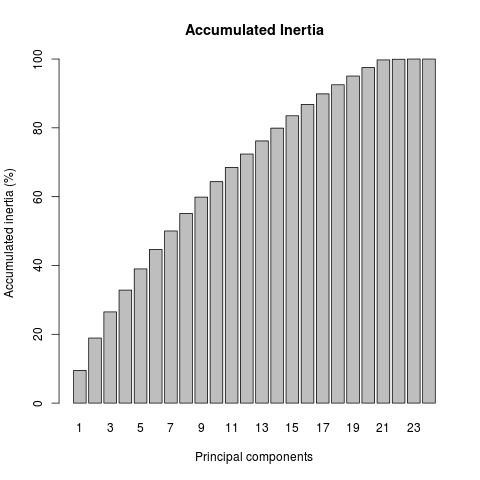
\includegraphics[width=3.5in]{images/ACP/a-cummulated-inertia-barplot.png}
\captionof{figure}{Accumulated percentage of inertia.}
\label{fig:boat1}
\end{center}

\subsection{Procedure}

Instead of coding an \textit{ad hoc} projection for some axis, what we did instead was systematically and programatically generating the projections for all the combinations of our 14 principal components. The code can be consulted in the appendix. However, for briefness, in this document we will only show the results for the first two iterations of our loop: 1-2 principal components (which explain about 20\% of the variance) as axis and 2-3 principal components as axis (which explain about 15\% of the variance). The explanation for what we did for 1-2 follows, but it applies for the 2-3 principal components too.

So, in order to proceed with PCA we will select the 2 principal components which explain most of the variance show in the figure~\ref{fig:boat1}, in our case component 1 and component 2 with 10\% and 20\% of accumulated inertia. As we were told in theory classes, with factorial analysis we want to find the most informative projection planes.

We have to take into account that in PCA the variable which has the highest contribution over the first factorial axis is the longest one among those projection with small angle to axis. Also, if two modalities of qualitative variables project close in the factorial space it means that these modalities are associated.

We plotted a projection of all numerical variables in order to observe the behavior of the variance between our variables. Also we selected which in our opinion were the most important qualitative variable as far as our study was concerned (\textit{match}; remember that our goal was to study what makes a date successful) and plotted all the different levels projected with our numerical two principal components, with the aim of observing how these variables were related with the variance of our numerical values. Then we did the same but with the categorical variables.

\subsection{Results}
As we can observe in figure~\ref{fig:indiv} we have 2 groups centered in the Y origin, also we can notice that whereas the variance increases values start to scatter from the origin point.
\begin{center}
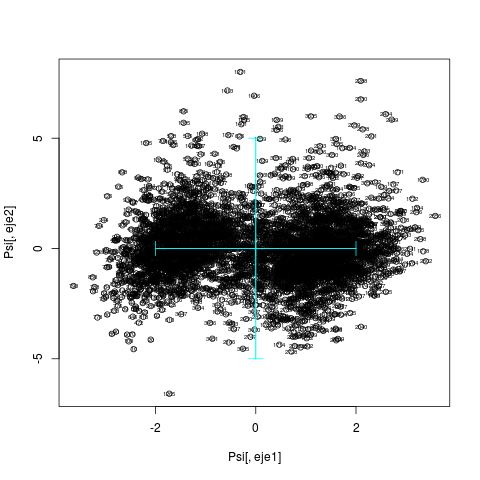
\includegraphics[width=3.5in]{images/ACP/individuals.png}
\captionof{figure}{Individuals projection of our first principal components}
\label{fig:indiv}
\end{center}

In figure~\ref{fig:projnum} we have a zoomed projection of all numeric variables. We can observe that most of them are pretty close to 0 variance, but \textit{tuition} and \textit{mn\_sat} seem not to follow the other variables, because they are variables related to the degree of the participant, which is a qualitative variable. However, we can observe that \textit{tuition} and \textit{mn\_sat} are correlated as \textit{tuition} might depend on the \textit{mn\_sat} mark and people who did not went to the university have a 0 in both variables.

Also we can find that \textit{imprelig} is correlative with \textit{imprace}, which explains that people who gives a lot of importance to the partner's religious background also gives it to race background and vice versa. Another interesting information we can extract from the plot is that income does not seem to be quite related to any other variable (maybe a bit with age) which could tell us that the older people are the more money they earn. Finally we can also determine that people who gives a lot of importance to the attractiveness (\textit{pf\_o\_attr} does not give too much importance to intelligence ((\textit{pf\_o\_int}) and vice versa. In other words, these attributes are not related to each other. What is more, this relation is also noticeable with the rate given to all participants (\textit{attr\_o}, \textit{intel\_o}).

\begin{center}
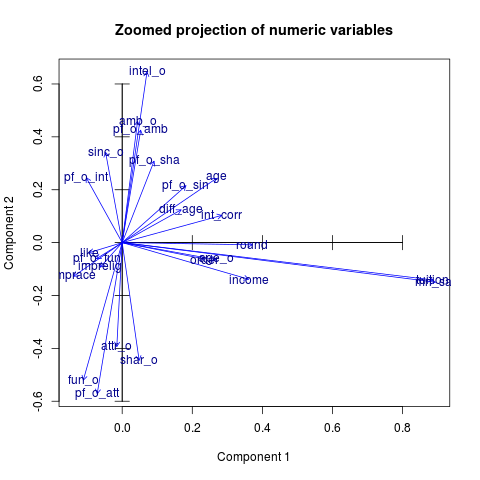
\includegraphics[width=5.5in]{images/ACP/projection_num_vars.png}
\captionof{figure}{All numerical variables projection.}
\label{fig:projnum}
\end{center}

Once we had checked how the numerical variables relate among each other, we plotted all qualitative variables projected together. In this plot we cannot perceive a clear relation between match and another qualitative, perhaps we can affirm that there is relation between the fact of being a female and having a match.

In figure~\ref{fig:projall} we projected the numerical to the previous plot, which gives us more information about the relation between categorical and numerical values. The qualitative variables of the legend in the upper left are the ordinal ones, the other ones are explained in the legend located in the bottom left.

In response to the initial question "Which attributes influence the selection of a romantic partner?" we can observe a clear relation between having a match (orange Y) and fun, having shared interests/hobbies and attractiveness. In contrast it seems that intelligence (\textit{intel\_o}) is not related with having a match. These results are pretty coherent with the ones observed in the bivariate analysis.

%\begin{center}
%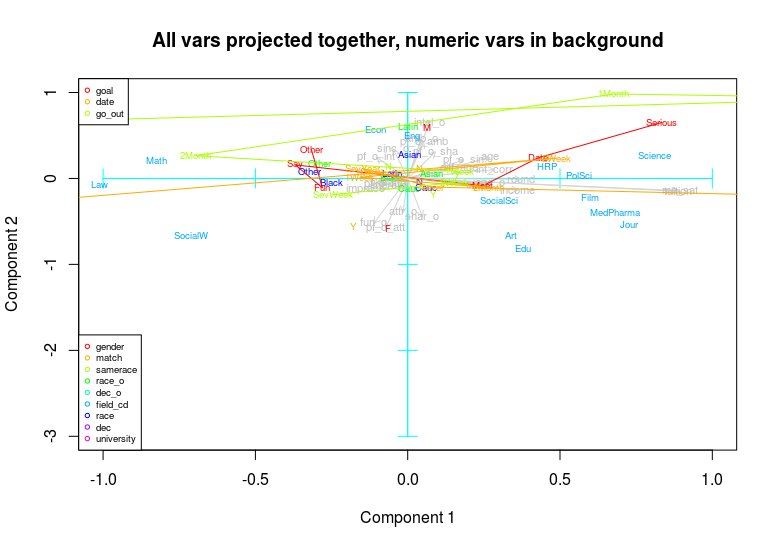
\includegraphics[width=3.5in]{images/ACP/all_together.png}
%\captionof{figure}{All qualitative variables projection.}
%\label{fig:projnum}
%\end{center}

\begin{figure}
  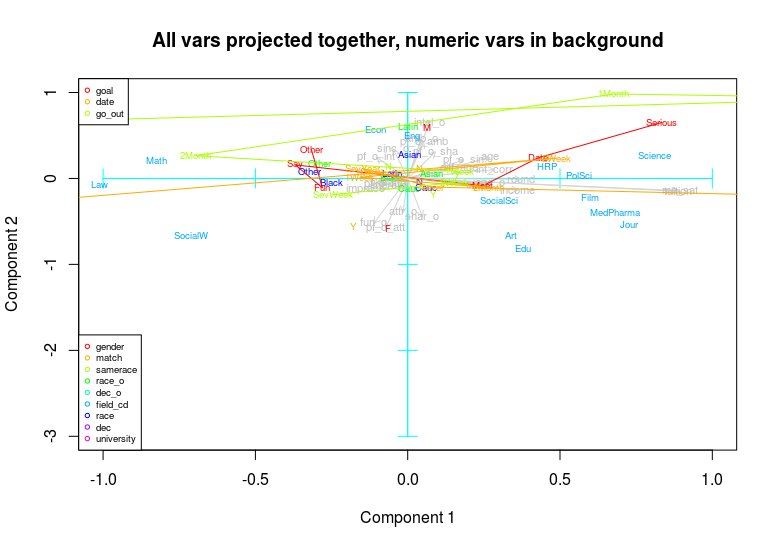
\includegraphics[width=\linewidth ,scale = 0.1]{images/ACP/all_together.png}
  \caption{All qualitative variables projection.}
  \label{fig:projall}
\end{figure}


In addition, we projected both cdgs of levels of the selected qualitative variable (\textit{match}) without representing the individual anymore:

\begin{center}
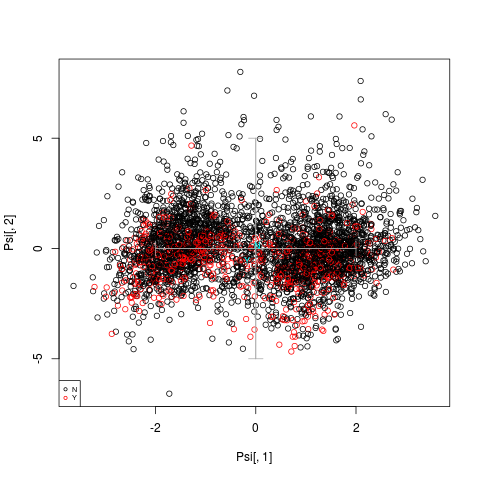
\includegraphics[width=3.5in]{images/ACP/x-1_y-2b-2-match-ill-proj.png}
\captionof{figure}{Match}
\label{fig:aLabelForReferencing}
\end{center}

\begin{center}
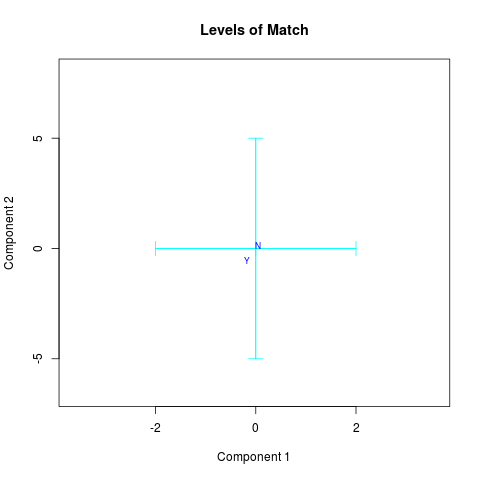
\includegraphics[width=3.5in]{images/ACP/x-1_y-2b-2-match.png}
\captionof{figure}{Match}
\label{fig:aLabelForReferencing}
\end{center}

\subsection{Extra results: principal components 2 and 3}

%As seen in figure~\ref{fig:boat1} our dataset has 24 principal component, we selected 14 (80\% of inertia) followed by analyzing a single iteration of the PCA algorithm (PC 1,2) which corresponds to the 20\% of accumulated inertia , but as our case has 14 pc we decided to also analyze pc(2,3), in order to have a better vision of how data is related.
As we can observe in figure~\ref{fig:boat2}, we have a single group centered in the (X,Y) origin. Also it is noticeable the fact that there is a group in the third sector which differs from the other points, as whereas the variance increases values start to scatter from the origin point. 
\begin{center}
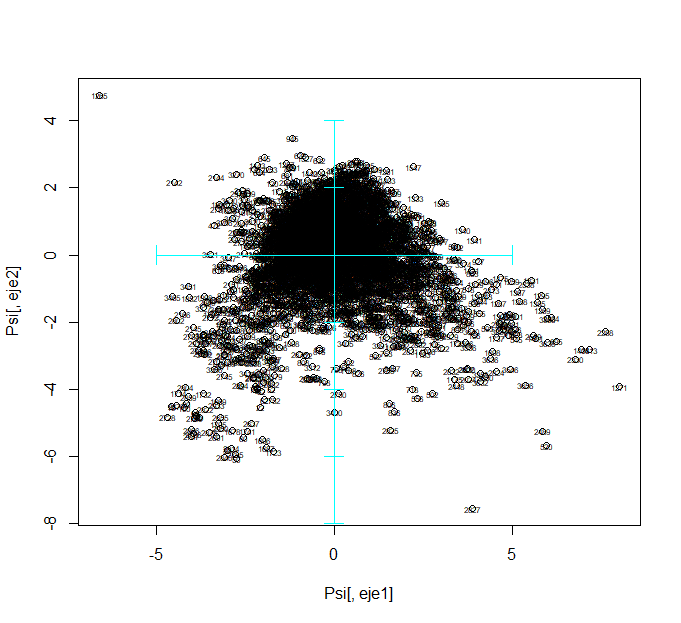
\includegraphics[width=3.5in]{images/ACP/2-3iteration/individuals-2-3.png}
\captionof{figure}{Accumulated percentage of inertia.}
\label{fig:boat2}
\end{center}

In our new zoomed projection of numeric variables we notice groups of variables that relate to each other. Notice how attributes variables(fun\_o, shar\_o...) are distributed among 2 groups (shar, fun, attr) and (amb, intel, sinc), and each group does not relate to the other. Finally we can also extract information about preferences, and how all preferences are related to each other.%some more than others, except pf\_o\_att which differs from the other.
\begin{center}
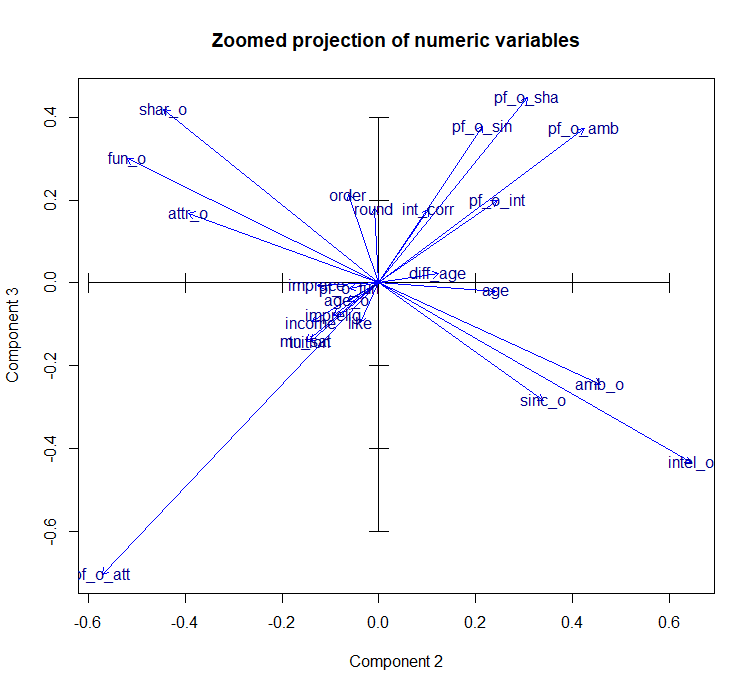
\includegraphics[width=5.5in]{images/ACP/2-3iteration/proj-all-nums-2-3.png}
\captionof{figure}{Zoomed projection of numeric variables}
\label{fig:numproj23}
\end{center}

The all variables projected plot \ref{fig:altog23} is quite different from the first one, but most of the relations noticed in the previous one still hold. However we can notice a relation between some field\_cd attributes, like Language, Social or medPharma which are quite related to having a match. This plot confirms the previous relations studied in the 1-2 iteration between having a match, being fun, and having shared interest/hobbies and attractiveness.
\begin{center}
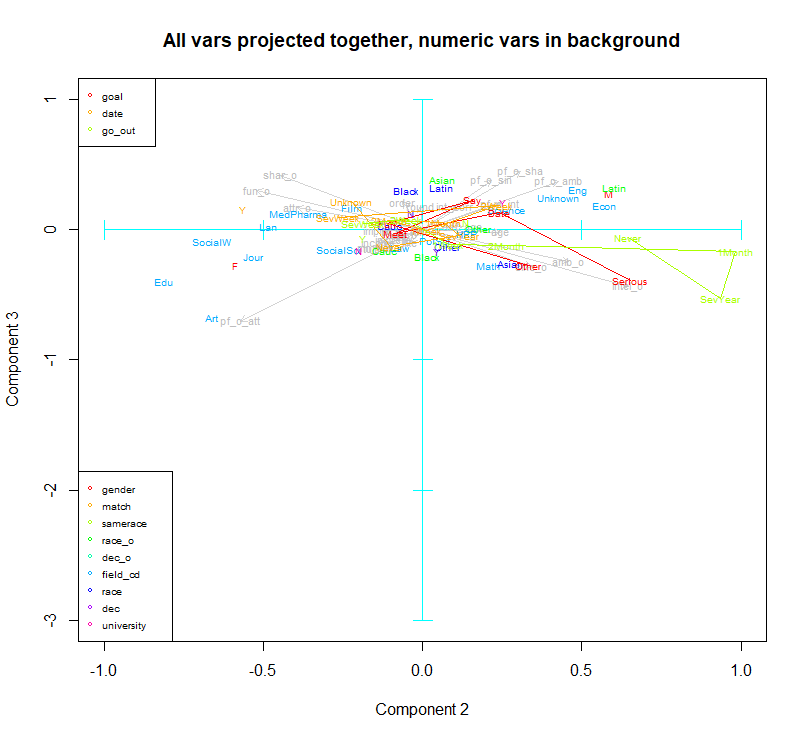
\includegraphics[width=\linewidth ,scale = 0.1]{images/ACP/2-3iteration/all-together-2-3.png}
\captionof{figure}{All vars projected together, numeric vars in background}
\label{fig:altog23}
\end{center}

\begin{center}
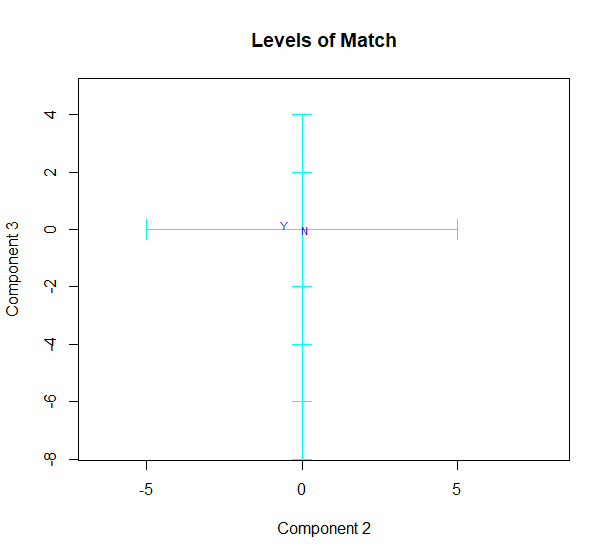
\includegraphics[width=3.5in]{images/ACP/2-3iteration/b-2-3-match.png}
\captionof{figure}{levels of match}
\label{fig:bmatch23}
\end{center}

\begin{center}
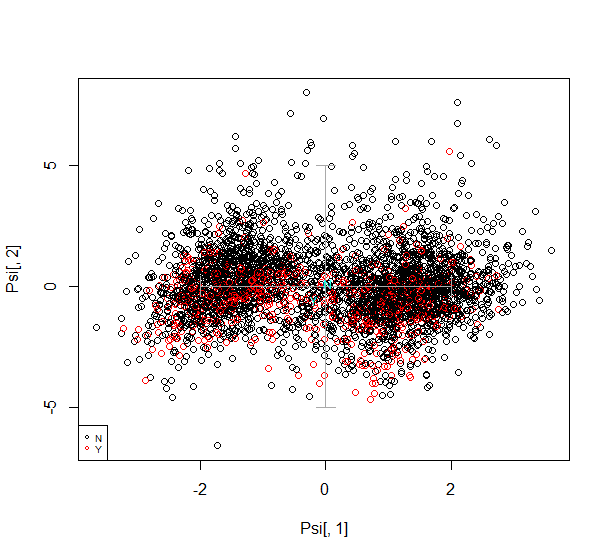
\includegraphics[width=3.5in]{images/ACP/2-3iteration/match-2-3.png}
\captionof{figure}{Match}
\label{fig:match23}
\end{center}

\end{document}